\documentclass[a4paper]{article}
\usepackage[a4paper,margin=0mm]{geometry}
\usepackage{fontspec}
\usepackage{unicode-math}
\usepackage{tikz}
\usepackage[table]{xcolor}
\usepackage[absolute]{textpos}
\usepackage{enumitem}
\usepackage{array}
\usepackage{multirow}

\setmainfont{Libertinus Serif}
\setsansfont{Libertinus Sans}
\setmathfont{Libertinus Math}
\newfontfamily\trackedsans{Libertinus Sans}[LetterSpace=8.0]

\definecolor{accent}{HTML}{602785}
\definecolor{badge}{HTML}{B8A0C8}
\definecolor{ink}{HTML}{2A2E30}

\setlength{\TPHorizModule}{1mm}
\setlength{\TPVertModule}{1mm}
\setlength{\parindent}{0pt}
\pagestyle{empty}

\newcommand{\LCOL}{16mm}
\newcommand{\RCOL}{111mm}
\newcommand{\COLW}{83mm}

\newcommand{\topicheader}[2]{%
\begin{textblock*}{194mm}(16mm,10mm)
\begin{tikzpicture}
\node[fill=accent,text=white,font=\sffamily\bfseries\fontsize{13}{13}\selectfont,
      minimum width=9mm,minimum height=9mm,inner sep=0pt] at (4.5mm,-4.5mm) {#1};
\node[font=\sffamily\bfseries\fontsize{15}{16}\selectfont,text=ink,anchor=west] at (12mm,-4.5mm) {#2};
\end{tikzpicture}
\end{textblock*}
\begin{textblock*}{194mm}(16mm,22.5mm)

\begin{tikzpicture}
\fill[accent] (0,0) rectangle (194mm,0.5mm);
\end{tikzpicture}
\end{textblock*}
}

\newcommand{\pagefooter}[1]{%
\begin{textblock*}{194mm}(8mm,286.41mm)
  
\begin{tikzpicture}
    \fill[accent] (0,0) rectangle (194mm,0.6mm);
  \end{tikzpicture}
\end{textblock*}
\begin{textblock*}{63.59mm}(8mm,288.27mm)
  {\sffamily\bfseries\color{accent}\fontsize{13}{16}\selectfont SAT 1200+}
\end{textblock*}
\begin{textblock*}{10mm}(188mm,288.27mm)
  \centering{\sffamily\color{accent}\fontsize{14}{16}\selectfont #1}
\end{textblock*}
}

\newcommand{\colrule}[2]{%
\begin{textblock*}{1mm}(105mm,#1mm)
\begin{tikzpicture}
\draw[black!65,line width=0.5pt] (0,0) -- (0,#2mm);
\end{tikzpicture}
\end{textblock*}
}

\newcommand{\setkicker}[2]{%
{\sffamily\bfseries\fontsize{12}{14}\selectfont #1.}\ {\itshape\fontsize{11}{14}\selectfont\color{black!75} #2}\par\vspace{2mm}%
}

\setlength{\fboxsep}{1.4pt}
\setlength{\fboxrule}{0.5pt}
\newcommand{\pnum}[1]{\fcolorbox{ink}{white}{\sffamily\bfseries\fontsize{8}{8}\selectfont #1}~}

\newcommand{\qrbox}[1]{%
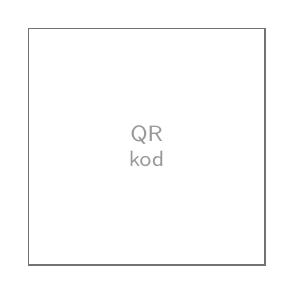
\begin{tikzpicture}
\draw[black!55,line width=0.6pt] (0,0) rectangle (30mm,30mm);
\node[black!40,font=\sffamily\fontsize{8}{9}\selectfont,align=center] at (15mm,15mm) {QR\\kod};
\end{tikzpicture}\\[1.5mm]
{\sffamily\fontsize{9}{11}\selectfont\color{black!70} #1}%
}

\arrayrulecolor{accent}
\setlength{\arrayrulewidth}{0.7pt}
\renewcommand{\arraystretch}{1.35}
\newcommand{\anstitle}[1]{{\sffamily\bfseries\color{accent}\fontsize{11}{13}\selectfont #1}\\[1.3mm]}

% ---- Minimal right-triangle diagram: #1 = right-angle vertex label (at origin),
% #2 = horizontal-leg vertex label, #3 = vertical-leg vertex label ----
\newcommand{\righttriangle}[3]{%
\begin{tikzpicture}[baseline=0mm]
\coordinate (R) at (0,0);
\coordinate (H) at (18mm,0);
\coordinate (V) at (0,14mm);
\draw[ink,thick] (V) -- (R) -- (H) -- cycle;
\draw[ink] (0,2.2mm) -- (2.2mm,2.2mm) -- (2.2mm,0);
\node[font=\small,below left] at (R) {#1};
\node[font=\small,right] at (H) {#2};
\node[font=\small,above] at (V) {#3};
\end{tikzpicture}%
}

\begin{document}

% ================= PAGE 1: Set 1 (ID sides, with diagrams) | Set 2 (exact ratios) =================
\topicheader{22}{To'g'ri Burchakli Uchburchak Trigonometriyasi}
\pagefooter{118}
\colrule{32}{238}
\mbox{}%

\begin{textblock*}{\COLW}(\LCOL,32mm)
{\fontsize{10.5}{13}\selectfont
\setkicker{1-to'plam}{Har bir uchburchak va burchak uchun qarshi tomon, qo'shni tomon va gipotenuzani ayting.}

\righttriangle{C}{B}{A}\\[2mm]
\noindent\pnum{1} Burchak $A$ uchun: \dotfill\\[5mm]
\noindent\pnum{2} Burchak $B$ uchun (xuddi shu uchburchak): \dotfill\\[8mm]

\righttriangle{Q}{R}{P}\\[2mm]
\noindent\pnum{3} Burchak $P$ uchun: \dotfill\\[5mm]
\noindent\pnum{4} Burchak $R$ uchun (xuddi shu uchburchak): \dotfill\\[8mm]

\righttriangle{Y}{Z}{X}\\[2mm]
\noindent\pnum{5} Burchak $X$ uchun: \dotfill\\[5mm]
\noindent\pnum{6} Burchak $Z$ uchun (xuddi shu uchburchak): \dotfill
}
\end{textblock*}

\begin{textblock*}{\COLW}(\RCOL,32mm)
{\fontsize{11}{14}\selectfont
\setkicker{2-to'plam}{Har bir uchburchak uchun $\sin\theta$, $\cos\theta$, $\tan\theta$ ni toping (kasrni soddalashtiring).}

\noindent\pnum{1} Katetlar $3$ va $4$, gipotenuza $5$. $\theta$ -- uzunligi $3$ bo'lgan katetga qarshi.\\[13mm]
\noindent\pnum{2} Xuddi shu uchburchak. $\theta$ -- uzunligi $4$ bo'lgan katetga qarshi.\\[13mm]
\noindent\pnum{3} Katetlar $5$ va $12$, gipotenuza $13$. $\theta$ -- uzunligi $5$ bo'lgan katetga qarshi.\\[13mm]
\noindent\pnum{4} Xuddi shu uchburchak. $\theta$ -- uzunligi $12$ bo'lgan katetga qarshi.\\[13mm]
\noindent\pnum{5} Katetlar $8$ va $15$, gipotenuza $17$. $\theta$ -- uzunligi $8$ bo'lgan katetga qarshi.\\[13mm]
\noindent\pnum{6} Katetlar $7$ va $24$, gipotenuza $25$. $\theta$ -- uzunligi $24$ bo'lgan katetga qarshi.
}
\end{textblock*}

\clearpage

% ================= PAGE 2: Set 3 (missing side) | Set 4 (missing angle) =================
\topicheader{22}{To'g'ri Burchakli Uchburchak Trigonometriyasi}
\pagefooter{119}
\colrule{32}{238}
\mbox{}%

\begin{textblock*}{\COLW}(\LCOL,32mm)
{\fontsize{11}{14}\selectfont
\setkicker{3-to'plam}{Etishmayotgan tomonni toping (yuzdan birigacha yaxlitlang).}

\noindent\pnum{1} Gipotenuza $=12$, burchak $=25°$. Qarshi tomonni toping.\\[13mm]
\noindent\pnum{2} Gipotenuza $=18$, burchak $=40°$. Qo'shni tomonni toping.\\[13mm]
\noindent\pnum{3} Qo'shni $=10$, burchak $=55°$. Qarshi tomonni toping.\\[13mm]
\noindent\pnum{4} Qarshi $=9$, burchak $=32°$. Gipotenuzani toping.\\[13mm]
\noindent\pnum{5} Gipotenuza $=22$, burchak $=63°$. Qo'shni tomonni toping.\\[13mm]
\noindent\pnum{6} Qo'shni $=14$, burchak $=47°$. Gipotenuzani toping.
}
\end{textblock*}

\begin{textblock*}{\COLW}(\RCOL,32mm)
{\fontsize{11}{14}\selectfont
\setkicker{4-to'plam}{Etishmayotgan burchakni toping (o'ndan birigacha yaxlitlang).}

\noindent\pnum{1} Qarshi $=6$, gipotenuza $=14$. Burchakni toping.\\[13mm]
\noindent\pnum{2} Qo'shni $=9$, gipotenuza $=20$. Burchakni toping.\\[13mm]
\noindent\pnum{3} Qarshi $=11$, qo'shni $=15$. Burchakni toping.\\[13mm]
\noindent\pnum{4} Qarshi $=18$, gipotenuza $=30$. Burchakni toping.\\[13mm]
\noindent\pnum{5} Qo'shni $=21$, qarshi $=25$ (bir xil burchakka nisbatan). Burchakni toping.\\[13mm]
\noindent\pnum{6} Qo'shni $=13$, gipotenuza $=37$. Burchakni toping.
}
\end{textblock*}

\clearpage

% ================= PAGE 3: Set 5 (applied word problems) | Set 6 (spot the error) =================
\topicheader{22}{To'g'ri Burchakli Uchburchak Trigonometriyasi}
\pagefooter{120}
\colrule{32}{238}
\mbox{}%

\begin{textblock*}{\COLW}(\LCOL,32mm)
{\fontsize{10.3}{13}\selectfont
\setkicker{5-to'plam}{Aralash amaliy masalalar (boshqacha ko'rsatilmasa, yuzdan birigacha yaxlitlang).}

\noindent\pnum{1} $12$ fut uzunlikdagi narvon devorga $68°$ burchak ostida tiralgan. U devorning qancha balandligiga yetadi?\\[9mm]
\noindent\pnum{2} Pandus gorizontal $40$ fut masofada $10°$ burchak ostida ko'tariladi. Pandusning o'zi (gipotenuza) qancha uzun?\\[9mm]
\noindent\pnum{3} Minoradan $100$ m masofadagi nuqtadan minora cho'qqisiga ko'tarilish burchagi $38°$. Minoraning balandligini toping.\\[9mm]
\noindent\pnum{4} Uçurtma ipi $65$ m uzunlikda va yer bilan $50°$ burchak hosil qiladi. Uçurtma odamdan gorizontal qancha uzoqda?\\[9mm]
\noindent\pnum{5} To'g'ri burchakli uchburchakning katetlari $9$ va $12$. Avval gipotenuzani, so'ng $9$ uzunlikdagi katetga qarshi burchakni toping (o'ndan birigacha).\\[9mm]
\noindent\pnum{6} Samolyot $6°$ pasayish burchagi ostida $2000$ m gorizontal masofani bosib o'tadi. Balandligi necha metrga kamayadi?
}
\end{textblock*}

\begin{textblock*}{\COLW}(\RCOL,32mm)
{\fontsize{10}{13}\selectfont
\setkicker{6-to'plam}{Xatoni toping -- buzilgan qadamni ayting, to'g'ri javobni bering.}

\noindent\pnum{1} To'g'ri burchak $C$ da, $BC=5$, $AC=12$, $AB=13$. $\sin A$ ni toping.\\[1mm]
\hspace*{7mm}\textit{``$\sin A=\frac{12}{13}$, chunki $12$ -- uzunroq katet.''}\\[2mm]
\hspace*{7mm}Xato va to'g'ri javob: \makebox[50mm]{\dotfill}\\[6mm]

\noindent\pnum{2} Xuddi shu uchburchak. $\cos B$ ni toping.\\[1mm]
\hspace*{7mm}\textit{``Burchak $A$ uchun qo'shni $AC=12$ edi, shuning uchun $\cos B=\frac{12}{13}$ ham.''}\\[2mm]
\hspace*{7mm}Xato va to'g'ri javob: \makebox[50mm]{\dotfill}\\[6mm]

\noindent\pnum{3} $\sin 30°$ ni toping.\\[1mm]
\hspace*{7mm}\textit{``Kalkulyatorga $30$ ni kiritib, $\sin 30\approx-0.988$ chiqdi.''}\\[2mm]
\hspace*{7mm}Xato va to'g'ri javob: \makebox[50mm]{\dotfill}\\[6mm]

\noindent\pnum{4} $\sin\theta=0.6$ berilgan, $\theta$ ni toping.\\[1mm]
\hspace*{7mm}\textit{``$\sin\theta=0.6$, shuning uchun $\theta=0.6°$.''}\\[2mm]
\hspace*{7mm}Xato va to'g'ri javob: \makebox[50mm]{\dotfill}\\[6mm]

\noindent\pnum{5} Gipotenuza $10$, bir katet $6$. Boshqa katetni toping.\\[1mm]
\hspace*{7mm}\textit{``$10^2+6^2=$boshqa katet$^2$, demak $\sqrt{136}\approx11.66$.''}\\[2mm]
\hspace*{7mm}Xato va to'g'ri javob: \makebox[50mm]{\dotfill}
}
\end{textblock*}

\clearpage

% ================= PAGE 4: Set 7 (bonus) =================
\topicheader{22}{To'g'ri Burchakli Uchburchak Trigonometriyasi}
\pagefooter{121}
\colrule{32}{238}
\mbox{}%

\begin{textblock*}{\COLW}(\LCOL,32mm)
{\fontsize{10.3}{13}\selectfont
\setkicker{7-to'plam}{Bonus / qiyin.}

\noindent\pnum{1} $\sin 23°\approx0.3907$ berilgan, $\cos 67°$ ni qaytadan hisoblamay toping (qo'shimcha burchak ayniyatidan foydalaning).\\[13mm]
\noindent\pnum{2} To'g'ri burchakli uchburchakning o'tkir burchaklaridan biri $34°$. Ikkinchi o'tkir burchakni toping va $\sin 34°$ bilan o'sha burchak kosinusi orasidagi bog'lanishni ayting.\\[13mm]
\noindent\pnum{3} Gipotenuza $26$, o'tkir burchaklardan biri $42°$. Ikkala katetni toping (yuzdan birigacha).\\[16mm]
\noindent\pnum{4} $20$ futlik narvon devorga $16$ fut balandlikda yetib boradi. Toping: (a) narvonning yer bilan hosil qilgan burchagi, (b) devor bilan hosil qilgan burchagi, (c) ikkala burchak qo'shimcha ekanini tasdiqlang.\\[16mm]
\noindent\pnum{5} Samolyot $15°$ doimiy burchak ostida $5000$ m uchish yo'li bo'ylab ko'tariladi. Bosib o'tilgan gorizontal masofa va erishilgan balandlikni toping (har birini yuzdan birigacha).
}
\end{textblock*}

\clearpage

% ================= PAGE 5: Javoblar -- full-page unified answer table =================
\topicheader{22}{To'g'ri Burchakli Uchburchak Trigonometriyasi}
\pagefooter{122}
\mbox{}%

\begin{textblock*}{194mm}(16mm,30mm)
{\bfseries\itshape\color{accent}\fontsize{19}{21}\selectfont\centering Javoblar\par}
\end{textblock*}

\begin{textblock*}{194mm}(16mm,42mm)
{\fontsize{8.7}{10.8}\selectfont
\centering
\renewcommand{\arraystretch}{1.25}
\begin{tabular}{|>{\centering\arraybackslash}p{24mm}|>{\centering\arraybackslash}p{8mm}|>{\centering\arraybackslash}p{136mm}|}
\hline
\rowcolor{badge!55}\textbf{To'plam} & \textbf{\#} & \textbf{Javob}\\
\hline
\multirow{6}{24mm}{\centering 1-to'plam} & 1 & Qarshi $=BC$, qo'shni $=AC$, gipotenuza $=AB$\\\cline{2-3}
 & 2 & Qarshi $=AC$, qo'shni $=BC$, gipotenuza $=AB$\\\cline{2-3}
 & 3 & Qarshi $=QR$, qo'shni $=PQ$, gipotenuza $=PR$\\\cline{2-3}
 & 4 & Qarshi $=PQ$, qo'shni $=QR$, gipotenuza $=PR$\\\cline{2-3}
 & 5 & Qarshi $=YZ$, qo'shni $=XY$, gipotenuza $=XZ$\\\cline{2-3}
 & 6 & Qarshi $=XY$, qo'shni $=YZ$, gipotenuza $=XZ$\\\hline
\multirow{6}{24mm}{\centering 2-to'plam} & 1 & $\sin=\frac35,\ \cos=\frac45,\ \tan=\frac34$\\\cline{2-3}
 & 2 & $\sin=\frac45,\ \cos=\frac35,\ \tan=\frac43$\\\cline{2-3}
 & 3 & $\sin=\frac{5}{13},\ \cos=\frac{12}{13},\ \tan=\frac{5}{12}$\\\cline{2-3}
 & 4 & $\sin=\frac{12}{13},\ \cos=\frac{5}{13},\ \tan=\frac{12}{5}$\\\cline{2-3}
 & 5 & $\sin=\frac{8}{17},\ \cos=\frac{15}{17},\ \tan=\frac{8}{15}$\\\cline{2-3}
 & 6 & $\sin=\frac{24}{25},\ \cos=\frac{7}{25},\ \tan=\frac{24}{7}$\\\hline
\multirow{6}{24mm}{\centering 3-to'plam} & 1 & $5.07$\\\cline{2-3}
 & 2 & $13.79$\\\cline{2-3}
 & 3 & $14.28$\\\cline{2-3}
 & 4 & $16.98$\\\cline{2-3}
 & 5 & $9.99$\\\cline{2-3}
 & 6 & $20.53$\\\hline
\multirow{6}{24mm}{\centering 4-to'plam} & 1 & $25.4°$\\\cline{2-3}
 & 2 & $63.3°$\\\cline{2-3}
 & 3 & $36.3°$\\\cline{2-3}
 & 4 & $36.9°$\\\cline{2-3}
 & 5 & $50.0°$\\\cline{2-3}
 & 6 & $69.4°$\\\hline
\multirow{6}{24mm}{\centering 5-to'plam} & 1 & $\approx11.13$ ft\\\cline{2-3}
 & 2 & $\approx40.62$ ft\\\cline{2-3}
 & 3 & $\approx78.13$ m\\\cline{2-3}
 & 4 & $\approx41.78$ m\\\cline{2-3}
 & 5 & Gipotenuza $=15$; burchak $\approx36.87°$\\\cline{2-3}
 & 6 & $\approx210.21$ m\\\hline
\multirow{5}{24mm}{\centering 6-to'plam} & 1 & Qarshi/qo'shni noto'g'ri aniqlangan. To'g'ri: $\sin A=\frac{5}{13}$.\\\cline{2-3}
 & 2 & Burchak almashganda tomonlar qayta aniqlanmagan. To'g'ri: $\cos B=\frac{5}{13}$.\\\cline{2-3}
 & 3 & Kalkulyator radian rejimida edi. To'g'ri: $\sin30°=0.5$.\\\cline{2-3}
 & 4 & Nisbat burchak deb olingan. To'g'ri: $\theta=\arcsin(0.6)\approx36.9°$.\\\cline{2-3}
 & 5 & Gipotenuza katet kabi qo'shilgan. To'g'ri: boshqa katet $=\sqrt{10^2-6^2}=8$.\\\hline
\multirow{5}{24mm}{\centering 7-to'plam} & 1 & $\cos67°=\sin23°\approx0.3907$\\\cline{2-3}
 & 2 & Boshqa burchak $=56°$; $\cos56°=\sin34°\approx0.5592$\\\cline{2-3}
 & 3 & Qarshi $\approx17.40$, qo'shni $\approx19.32$\\\cline{2-3}
 & 4 & (a) $\approx53.13°$, (b) $\approx36.87°$, (c) $53.13°+36.87°=90°$ (toʻgʻri)\\\cline{2-3}
 & 5 & Gorizontal $\approx4829.63$ m; balandlik $\approx1294.10$ m\\\hline
\end{tabular}
}
\end{textblock*}

\begin{textblock*}{194mm}(16mm,250mm)
\centering
{\sffamily\fontsize{9.5}{11.5}\selectfont\color{black!70} Video yechimlar va qo'shimcha testlar uchun quyidagi QR kodlarni skanerlang:}\\[4mm]
\begin{minipage}[t]{32mm}\centering\qrbox{YouTube}\end{minipage}%
\hspace{16mm}%
\begin{minipage}[t]{32mm}\centering\qrbox{Telegram}\end{minipage}
\end{textblock*}

\end{document}
